\begin{myposter}{
    Исследуемые модели
}

    \headerbox
    {Исследуемая модель с учетом инерции роликов}
    {name=first,column=0,row=0,span=3}
    {
        {\huge\bf
            \begin{figure}[H]
                \centering
                \minipage{0.45\textwidth}
                    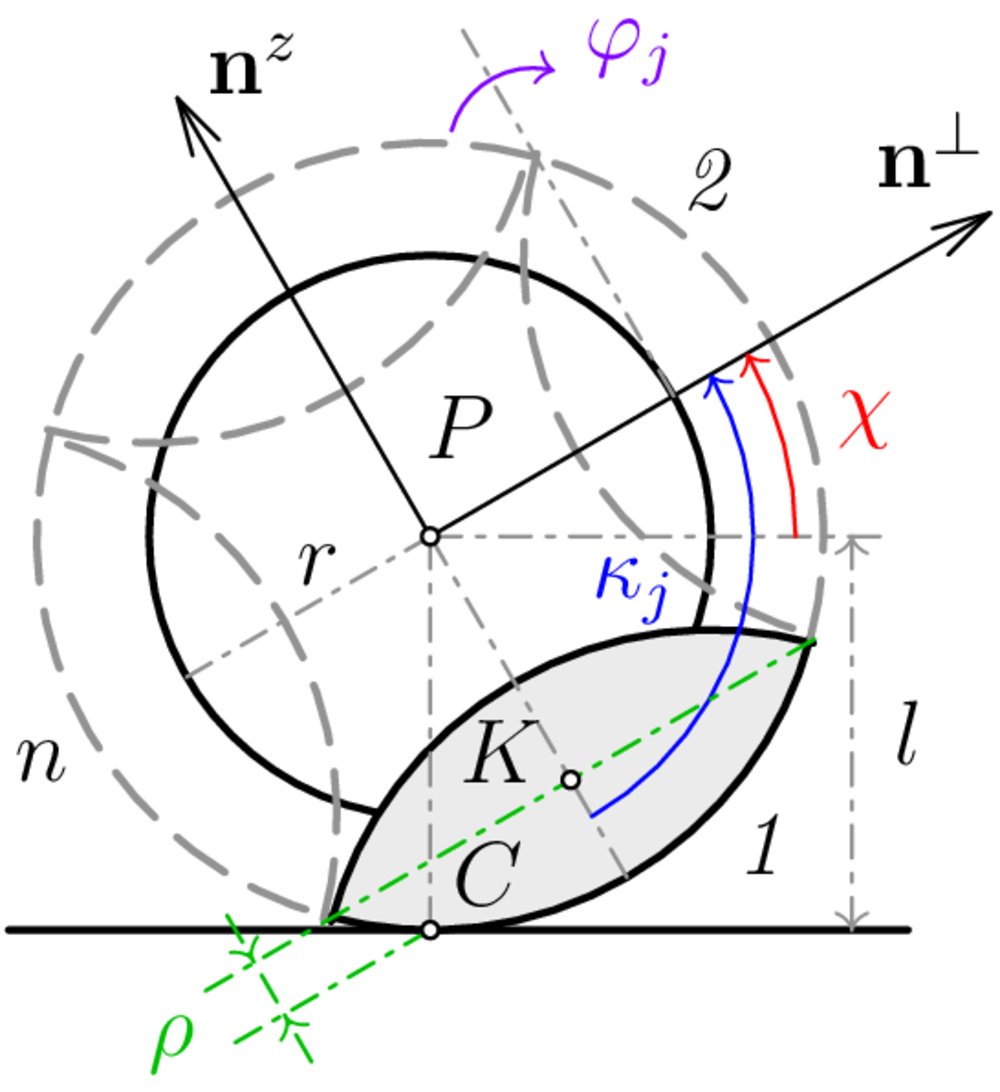
\includegraphics[width=0.8\textwidth]{content/pic/asypng/pic_wheel.png}
                    % \asyinclude{content/pic/asy/pic_wheel.asy}
                    % \caption{Колесо}
                \endminipage
                \qquad
                \minipage{0.45\textwidth}
                    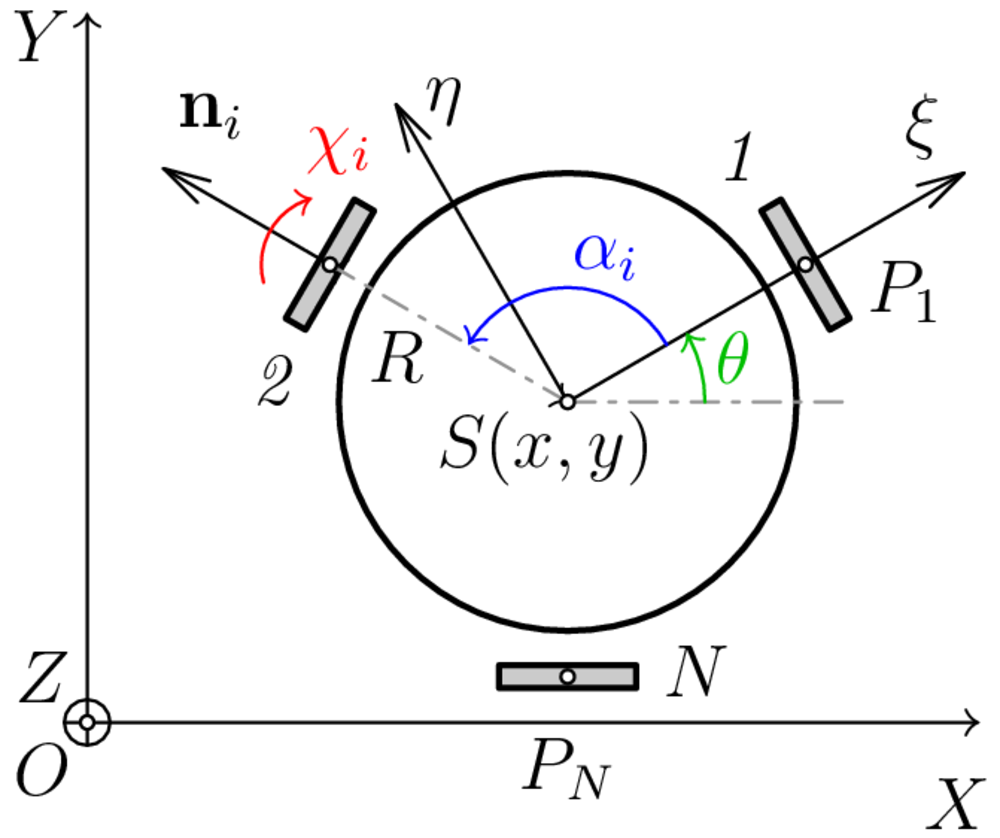
\includegraphics[width=1.05\textwidth]{content/pic/asypng/pic_cart.png}
                    % \asyinclude{content/pic/asy/pic_cart.asy}
                    % \caption{Экипаж}
                \endminipage
            \end{figure}
        }
    }
    
    \headerbox
    {Модели контакта}
    {name=second,column=0,row=1,below=first,span=3}
    {
        {\huge\bf
            \vspace{10pt}
            \begin{itemize}
                \item {
                    Главы 1 и 2. Абсолютно шероховатая плоскость
                    \begin{itemize}
                        \item {
                            Скорости точек контакта равны нулю:
                            $$ \vec{v}_{C_i} = 0, \quad i = 1 \dots N $$
                        }
                        \item {
                            Количество степеней свободы
                            $$ 3 + N(n-1) $$
                        }
                    \end{itemize}
                }
                \item {
                    Глава 3. Плоскость с трением
                    \begin{itemize}
                        \item {
                            Вязкое трение
                            $$
                                \vec{F} = -\gamma\vec{v}_{C_i}
                            $$
                        }
                        \item {
                            Регуляризованное сухое трение
                            $$
                                \vec{F} = -\mu N \vec{v}_{C_i}
                                    \left\{
                                        \begin{array}{ll}
                                            \ddfrac{1}{\delta}, \enspace |\vec{v}_{C_i}| < \delta \ll 1 \vspace{7pt}\\
                                            \ddfrac{1}{|\vec{v}_{C_i}|}\enspace \text{иначе}
                                        \end{array}
                                    \right.
                            $$
                        }
                        \item {
                            Количество степеней свободы:
                            $$ 3 + N(n + 1) $$
                        }
                    \end{itemize}
                }
            \end{itemize}
            \vspace{10pt}
        }
    }

\end{myposter}
